\documentclass{article}
\usepackage{../cs170}
\usepackage[version=4]{mhchem}
\AtBeginDocument{\RenewCommandCopy\qty\SI}

\def\title{HW 06}

\begin{document}

\maketitle

\question{}

\begin{subparts}
  \item Mean free time, measured in [\unit{\second}], refers to the average time a particle spends traveling before colliding with another particle within a substance.
  \item Mobility, measured in [\unit{\meter\squared\per\volt\per\second}], is a measure of how much velocity a particle attains when placed in an electric field.
  \item
  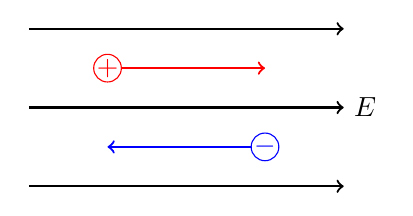
\begin{tikzpicture}
      \draw[black, thick, ->] (-1, 0) -- (3, 0);
      \draw[black, thick, ->] (-1, 1) -- (3, 1) node[anchor=west]{\(\bm{E}\)};
      \draw[black, thick, ->] (-1, 2) -- (3, 2);
      \draw[blue, thick, ->] (2, 0.5) -- (0, 0.5);
      \draw[color=blue, fill=white] (2, 0.5) circle (5pt) node[text=blue]{\(-\)};
      \draw[red, thick, ->] (0, 1.5) -- (2, 1.5);
      \draw[color=red, fill=white] (0, 1.5) circle (5pt) node[text=red]{\(+\)};
  \end{tikzpicture}
  \item Given a silicon bar of length \(L\) with a voltage \(V\) applied to it, the strength of the electric field \(E\) is defined as \(E = \frac{V}{L}\).
\end{subparts}

\question{}

\begin{subparts}
  \item The Pauli exclusion principle states that no two particles can occupy the same quantum state (i.e. spin, charge, position).
  \item
  \begin{enumerate}
    \item \ce{Si}: 4 valence electrons
    \item \ce{Ge}: 4 valence electrons
    \item \ce{As}: 5 valence electrons
    \item \ce{B}: 3 valence electrons
    \item \ce{P}: 5 valence electrons
  \end{enumerate}
  \item With respect to the energy bands, metals have very small band gaps between energy bands, meaning it is easy for electrons to jump to higher energy bands.
  Likewise, semiconductors have slightly larger band gaps, and insulators have very large band gaps.
  \item Free electrons refer to electrons that have been ionized out of a semiconductor, and ``holes'' refer to the local positive charge created by the lack of an electron.
\end{subparts}

\question{}

If we apply an electric field to a sample of silicon at \qty{0}{\kelvin}, it's unlikely any current is induced, since most of the electrons will be in the ground state band.
If we apply an electric field at \qty{300}{\kelvin}, a small but significant current will be induced, since more electrons will be in conduction bands, since \(U = kT\).
At \qty{1000}{\kelvin}, the current induced will be stronger due to even higher energies.

\question{}

\begin{subparts}
  \item The lattice constant of silicon is \qty{5.431020511}{\angstrom}.
  \item There are \(8\) silicon atoms in a unit cell.
  \item The atomic density of silicon is \(\frac{\qty{2.3296}{\cancel\gram}}{\qty{1}{\cancel\centi\meter\cubed}} \cdot \frac{\qty{1}{\mole}}{\qty{28.085}{\cancel\gram}} \cdot \frac{\qty{1e6}{\cancel\centi\meter\cubed}}{\qty{1}{\meter\cubed}} \cdot N_A = \qty{4.995e28}{\per\meter\cubed}\)
  \item The number of silicon atoms is \(\qty{20}{\nano\meter} \cdot \qty{40}{\nano\meter} \cdot \qty{10}{\nano\meter} \cdot \frac{\qty{1}{\cancel\meter\cubed}}{\qty{1e27}{\nano\meter\cubed}} \cdot \qty{4.995e28}{\cancel\per\meter\cubed} = \num{399620}\).
\end{subparts}

\question{}

One other semiconductor is \ce{UO_2}, or uranium dioxide.
Its bandgap is \qty{1.3}{\electronvolt}.
Its applications include high-voltage integrated circuits due to its high dielectric constant and in high-temperature electronic applications.

\end{document}
